\documentclass[letterpaper,12pt]{article}
\usepackage[parfill]{parskip}
\usepackage{multicol}
\usepackage{xcolor}
\usepackage{wrapfig}
\usepackage{subcaption}
\usepackage{mathtools}
\usepackage{enumitem}
\usepackage[backend=biber]{biblatex}
\addbibresource{references.bib}
\usepackage{float}
\usepackage{enumitem}
\setitemize{noitemsep,topsep=0pt,parsep=3pt,partopsep=0pt}
\usepackage{booktabs}
\usepackage{tabularx} % extra features for tabular environment
\usepackage{amsmath}  % improve math presentation
\usepackage{graphicx} % takes care of graphic including machinery
\usepackage{caption}
\usepackage[margin=2cm,letterpaper]{geometry} % decreases margins
\usepackage[final]{hyperref} % adds hyper links inside the generated pdf file
\hypersetup{
	colorlinks=true,       % false: boxed links; true: colored links
	linkcolor=gray,        % color of internal links
	citecolor=gray,        % color of links to bibliography
	filecolor=magenta,     % color of file links
	urlcolor=blue         
}
%++++++++++++++++++++++++++++++++++++++++

\title{\vspace{-2cm} Wing Analysis Final Report}
\author{\vspace{-1cm} Luca Owen-Jones [co438]}
\date{\vspace{-0.5cm} June 2026}

\begin{document}

\maketitle

Steps:
** All graphs need replacing, currently just screen grabs.

** Summary **

\section{Introduction}

\section{Discussion of model}
Brief description of the model, limitations?


Include the modified TE kutta condition

\section{Model validation}

\subsection{Panel number resolution}

To compare the variation of solution fidelity with panel number, results for Van de Vooren airfoil were compared. This airfoil geometry is obtained from conformal mapping of a cylinder, therefore an exact analytical solution exists.

This exact solution is plotted against the model output for various panel counts. The model is most inaccurate close to the suction peak where there is a large adverse pressure gradient. This inaccuracy is more pronounced for the 'thin' section than the 'thick', as the adverse pressure gradient experienced is higher. For panel counts larger than 400, the model output matches the exact solution sufficiently well; therefore, future investigations** will use 400 panels.

However, these results highlight a disadvantage of the model. Rather than using evenly spaced panels, it would be advantageous to increase the density close to the leading edge, where a higher resolution has a larger effect. This would allow a lower overall panel count while preserving accuracy, and is implemented in other, industry standard, panel method solvers.

**Plots for both thin and thick**

\subsection{Boundary layer validation}

The boundary layer solver is validated through comparison with the exact Blasius solution, valid for laminar flow in a zero pressure gradient. Until natural transition, which occurs at $\text{x/L} = 0.38$, the calculated momentum thickness ($\theta$ value) matches closely with Blasius.

\begin{figure}[H]
    \centering
    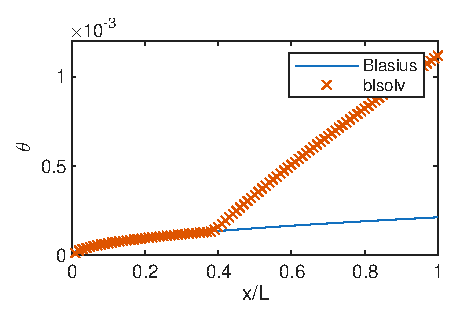
\includegraphics[width=0.8\linewidth]{../../Figures/bl_valid.eps}
    \caption{Comparison with the exact Blasius solution.}
    \label{fig:bl_valid}
\end{figure}

\subsection{Comparison with NACA 0012 and NACA 4412 foils}

Further validation is completed using two standard NACA airfoils: 0012 and 4412. Experimental data for these is widely available for comparison.




----------------------------
Testing of software on Naca 0012 and 4412 airfoils with plots. Can also use xfoil to compare. L obviously stays too high after stall.

Large number of questions on p30 of the handout to discuss here. 
Key issue in comparison of CL will be the lack of boundary layer consideration in calc of lift- does not consider stall





\subsection{Comparison with Xfoil}

Why Xfoil is better, industry standard panel method solver. Takes into account BL effects for lift etc, used in industry for inverse design.


\section{High L/D airfoil design}

Aim is high L/D, brief why, what are the considerations and trade-offs in trying to achieve this.

\subsection{Low Re design}

Starting point: \textbf{NACA0012}.

\begin{figure}[H]
    \centering
    
\includegraphics[width=1\linewidth]{0012 LD.jpeg}
    \caption{NACA0012}
    \label{fig:placeholder}
\end{figure}

\begin{figure}[H]
    \centering
    
\includegraphics[width=1\linewidth]{0012 LD ratio.jpeg}
    \caption{NACA0012. Max L/D = 58.82 at 7.6deg. Corresponding CL = 0.9145}
    \label{fig:placeholder}
\end{figure}

\begin{figure}[H]
    \centering
    
\includegraphics[width=1\linewidth]{0012 cp 7.6deg.png}
    \caption{NACA0012. cp at max angle of attack- early separation, turbulent attached over most of the chord.}
    \label{fig:placeholder}
\end{figure}

Decided to try to maintain laminar flow- lower drag. Increased the thickness to reduce the severity of the post suction peak adverse pressure gradient.

\textbf{LLL01} Increased thickness to 15\%, equivalent to the NACA 0015

\begin{figure}[H]
    \centering
    
\includegraphics[width=1\linewidth]{cp LLL01 4.9.jpeg}
    \caption{NACA0015.}
    \label{fig:placeholder}
\end{figure}

At 4.9 deg (max L/D), L/D 53.3, CL 0.605, so this is actually worse than NACA0012

\begin{figure}[H]
    \centering
    
\includegraphics[width=1\linewidth]{cp LLL01 7.6deg.jpeg}
    \caption{NACA0015.}
    \label{fig:placeholder}
\end{figure}

LLL01 at 7.6deg L/D 50.11, CL 0.937  

\begin{figure}[H]
    \centering
    
\includegraphics[width=1\linewidth]{CL CD LLL01.jpeg}
    \caption{NACA0015.}
    \label{fig:placeholder}
\end{figure}

cp characteristic actually doesnt seem much better, however now have a visible laminar bucket.

Centered around zero incidence (CL = 0 with no camber). Decided to try to increase L/D by increasing L in this low incidence region: adding camber.

\textbf{LLL02} 

Camber: moving the laminar bucket towards positive CL.
Added 2\% camber at 40\% chord.

Max L/D 78.8 at 6.1deg, CL 1.005

\begin{figure}[H]
    \centering
    
\includegraphics[width=1\linewidth]{CL CD LLL02.jpeg}
    \caption{LLL02}
    \label{fig:placeholder}
\end{figure}

\begin{figure}[H]
    \centering
    
\includegraphics[width=1\linewidth]{LLL02 cp 6.1deg.jpeg}
    \caption{LLL02}
    \label{fig:placeholder}
\end{figure}

However separation is still quite early

\textbf{LLL03}

Moving point of max thickness to 35\%

At best performing angle (6deg):

\begin{figure}[H]
    \centering
    
\includegraphics[width=1\linewidth]{cp 6deg LLL03.jpeg}
    \caption{LLL03 at 6deg}
    \label{fig:placeholder}
\end{figure}

\begin{figure}[H]
    \centering
    
\includegraphics[width=1\linewidth]{LLL03 CD CL.jpeg}
    \caption{}
    \label{fig:placeholder}
\end{figure}

\begin{figure}[H]
    \centering
    
\includegraphics[width=1\linewidth]{LD ratio LLL03.jpeg}
    \caption{this is for 400 panels}
    \label{fig:placeholder}
\end{figure}

Concerned about the jump shown in L/D, seems to be caused by the `wiggly' m plot. point of laminar separation suddenly jumps towards the leading edge


\textbf{LLL04}

Increasing camber to 4\%, moving max camber point back from 40\% to 50\%. Thickness still 15\%, max at 35\% chord.

LLL04 L/D 91.4 at 5.6deg, CL 1.26

\begin{figure}[H]
    \centering
    
\includegraphics[width=1\linewidth]{LD LLL04.jpeg}
    \caption{LLL04 with 800 panels. with 400 is looked like the jump in LLL03}
    \label{fig:placeholder}
\end{figure}

\begin{figure}[H]
    \centering
    
\includegraphics[width=1\linewidth]{LLL04 LD ratio.jpeg}
    \caption{LLL04}
    \label{fig:placeholder}
\end{figure}

\begin{figure}[H]
    \centering
    
\includegraphics[width=1\linewidth]{LLL04 5.6deg cp.jpeg}
    \caption{LLL04. 5.6deg cp}
    \label{fig:placeholder}
\end{figure}

\textbf{LLL05}

Continued to increase camber, increased to 7\% with max at 50\% chord. Thickness unchanged. Want the cp plot to be flatter near the leading edge.

\begin{figure}[H]
    \centering
    
\includegraphics[width=1\linewidth]{LLL05 cp 2.3deg.jpeg}
    \caption{LLL05}
    \label{fig:placeholder}
\end{figure}


Max at 2.3deg, L/D 100.435, CL 1.284

\begin{figure}[H]
    \centering
    
\includegraphics[width=1\linewidth]{LLL05 L D ratio.jpeg}
    \caption{LLL05}
    \label{fig:placeholder}
\end{figure}

\begin{figure}[H]
    \centering
    
\includegraphics[width=1\linewidth]{LLL05 L D.jpeg}
    \caption{LLL05}
    \label{fig:placeholder}
\end{figure}

-----------------------------------------------------
\textbf{LLL06}

Reduced thickness to 12\%


At 3.5deg

\begin{figure}[H]
    \centering
    
\includegraphics[width=1\linewidth]{LLL06 cp 3.5deg.png}
    \caption{LLL06}
    \label{fig:placeholder}
\end{figure}

\begin{figure}[H]
    \centering
    
\includegraphics[width=1\linewidth]{LLL06 LD ratio.png}
    \caption{LLL06}
    \label{fig:placeholder}
\end{figure}

\begin{figure}[H]
    \centering
    
\includegraphics[width=1\linewidth]{LLL06 LD.png}
    \caption{LLL06}
    \label{fig:placeholder}
\end{figure}

\textbf{LLL07}

Reduced thickness to 10\%

Further improvements

---------------------------------------------

Decided to try manipulating the geometry manually, rather than just camber and thickness, however had issues with using wasg, as the curves would stop being smooth and cause early separation- very sensitive. Tried to implement a least squares spline tool, however issues with the non monotonic variation of y with x- splitting the top and bottom into two different splines prevented smoothness at the leading edge, fixing this stopped the LE and TE being in the correct location. Decided to reduce the number of spline points to be manipulated instead. This also has the benefit of smoothing the cp plot.

\textbf{LLL06b}

Aiming to delay separation on the lower surface by reducing the curvature there (adjustments were near the trailing edge)

Managed to do this, although very little effect on L/D

\textbf{LLL07b}

Still very little improvement on L/D or location of separation point, but LE part of cp looks better

\textbf{LLL08b}

Trying to delay separation point. At LLL08b6 managed to achieve natural transition, however earlier turbulent separation. would be nice to fix this


\subsection{}




\section{Notes:}

(5) INcluding direct copy paste, needs rewording

Laminar boundary layers produce less skin friction drag, but more inclined to separate

Leading edge vs trailing edge separation, leading edge radius

Kutta condition only after the starting vortex is shed- circulation and lift- just interesting

Thin sections better for laminar flow, model aircraft often use turbulators

Transition depends on Re and roughness, needs to be manufactured to a precise profile, with a high standard of surface finish (more on this in chap 14). Also need to mainitain it in operational conditions.

NACA 6-series good for remaining laminar, need to operate in the CD 'bucket' region. Moving the position of maximum thickness rearward reduces min CD, but narrows the range of angle of attack over which low-drag laminar flow can be maintained. It also reduces the maximum lift coefficient that can be obtained. Reducing the thickness-to-chord ratio has a similar effect.

THicker airfoils have a larger range of low-drag operating conditions (wider bucket) with a higher max cl, at the expense of a slightly higher min CD. Can use spars to reduce weight.

Only apply to 2D sections as induced drag etc not considered.

NACA 6618 was designed inversely to have as flat an upper pressure distribution as possible, to allow laminar flow to be maintained. 

---------------

Ncrit- 'disturbance' already in the flow e.g. roughness, disturbed flow. typical wind tunnel is 9


\printbibliography
\end{document}
